\documentclass[border=1mm]{standalone}
% \usepackage[margin=2.5cm]{geometry}

\usepackage{graphicx,tikz,tikz-layers} 
\usetikzlibrary{decorations.markings,calc,positioning,arrows,shapes.geometric,arrows.meta,matrix}

\colorlet{myred}{red!80!black}
\colorlet{myblue}{blue!80!black}
\colorlet{mybluee}{myblue!80!black}
\colorlet{mygreen}{green!60!black}
\colorlet{myorange}{orange!70!red!60!black}
\colorlet{mydarkred}{red!20!black}
\colorlet{mydarkblue}{blue!40!black}
\colorlet{mydarkgreen}{green!20!black}


\begin{document}

% \resizebox{\textwidth}{!}{
\tikz[font=\small,scale=1, every node/.style={outer sep=0pt, inner sep=0pt, align=center}, w/.style={minimum width=#1},h/.style={minimum height=#1},s/.style={minimum size=#1}, eu/.style={shorten >=#1},ed/.style={shorten <=#1},line join=round]
{
\tikzset{>={Latex[length=1.5mm, width=1.25mm]}}

\node[draw] (im) {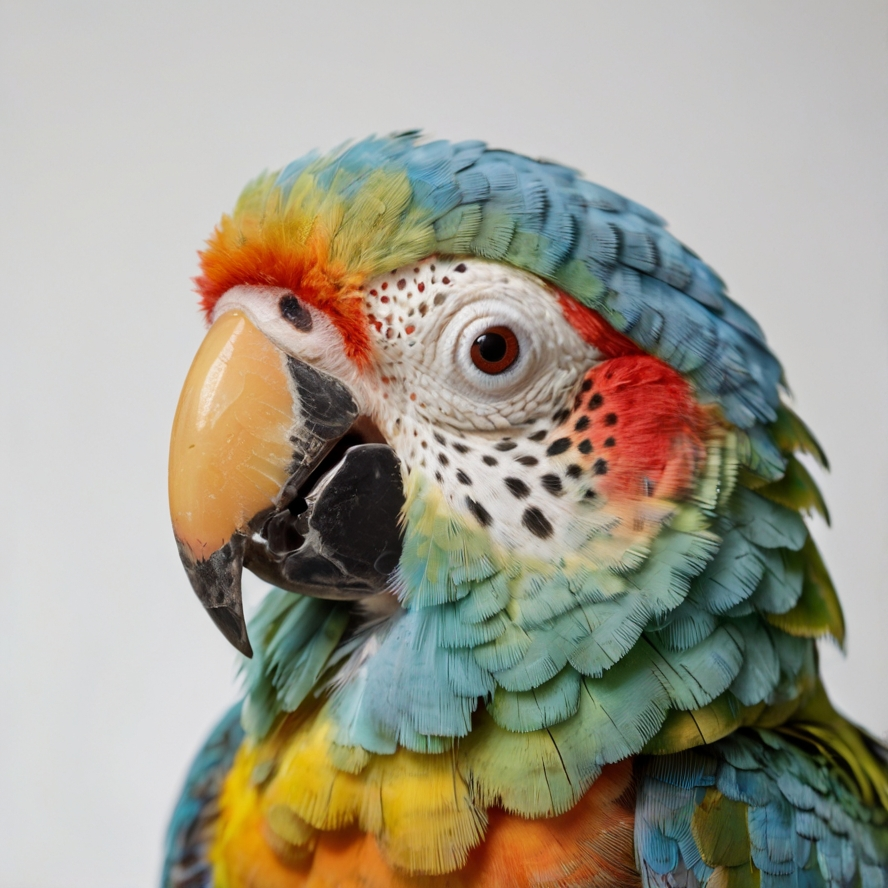
\includegraphics[width=2cm]{images/parrot3.jpg}};
\begin{scope}[on behind layer]
\node[draw] (lay1) at ($(im)+(-.1,.1)$) {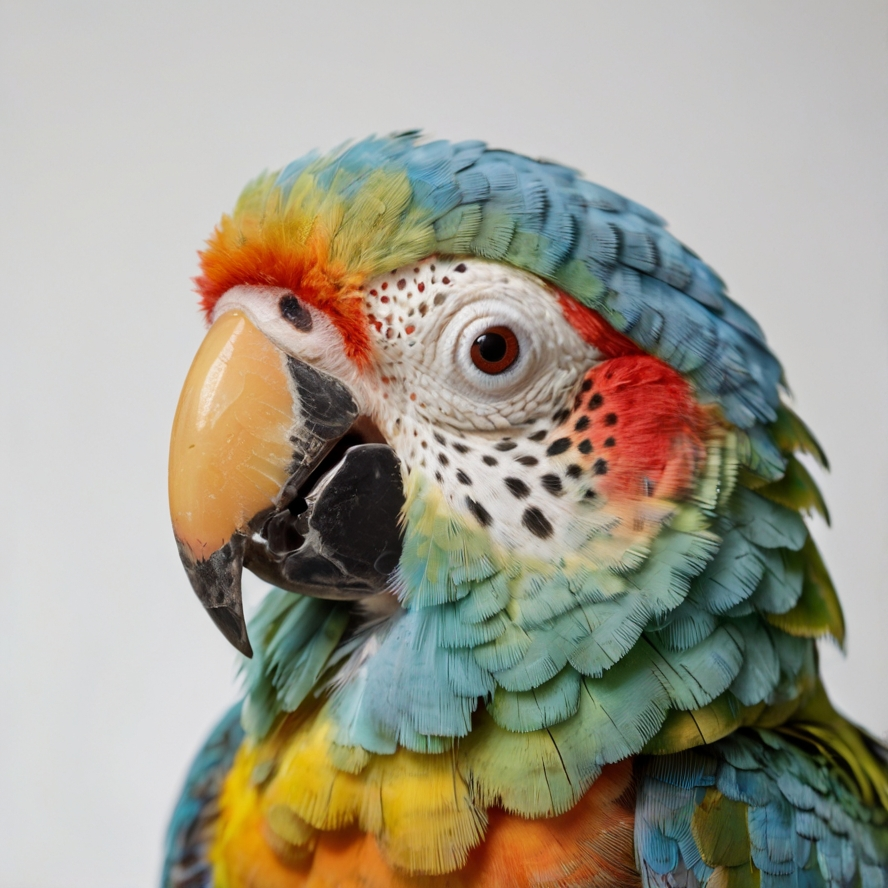
\includegraphics[width=2cm]{images/parrot3.jpg}};
\end{scope}
\begin{scope}[on background layer]
\node[draw] (lay2) at ($(lay1)+(-.1,.1)$) {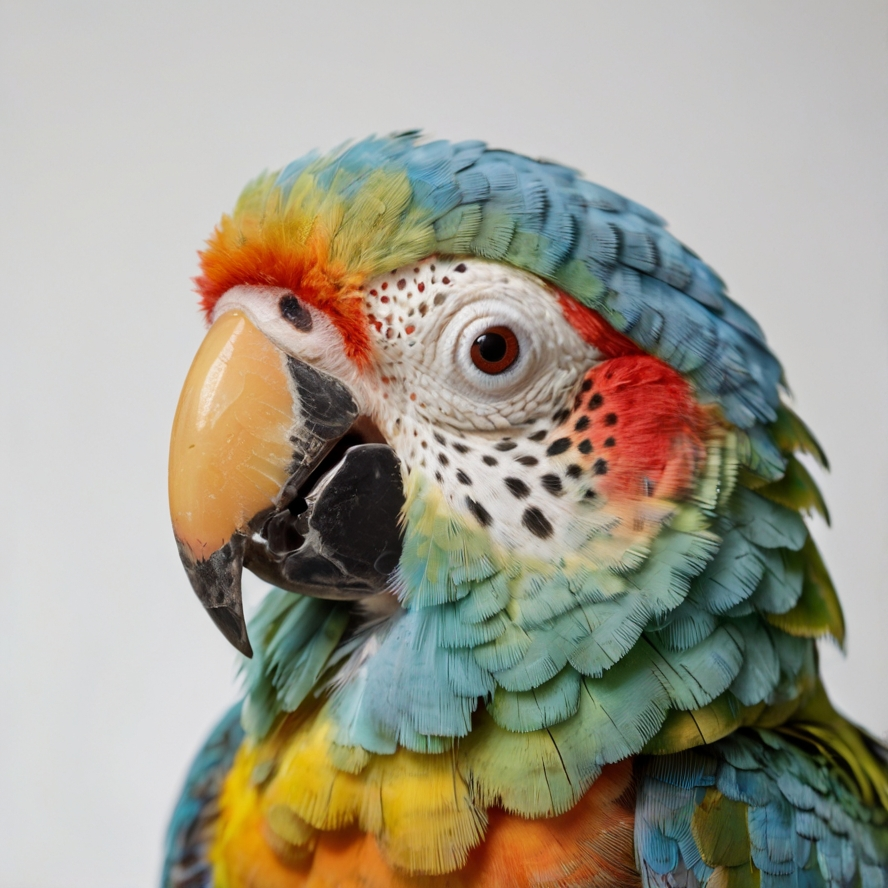
\includegraphics[width=2cm]{images/parrot3.jpg}};
\end{scope}

\node[w=2cm, h=2cm, right=1cm of im] (a) {Image\\Encoder};
\begin{scope}[on behind layer]
 \draw[fill=mygreen!15] (a.north west)--(a.south west)--($(a.south east)+(0,.3)$)--($(a.north east)+(0,-.3)$)--cycle;   
\end{scope}

%--
\node[draw, above=3cm of im, w=2cm, h=1cm, fill=white] (pta) {wild \\bird parrot};
\begin{scope}[on behind layer]
\node[draw, w=2cm, h=1cm, fill=white] (lay1) at ($(pta)+(-.1,.1)$) {};
\end{scope}
\begin{scope}[on background layer]
\node[draw, w=2cm, h=1cm, fill=white] (lay2) at ($(lay1)+(-.1,.1)$) {};
\end{scope}

\node[w=2cm, h=2cm, right=1cm of pta] (te1) {Text\\Encoder};
\begin{scope}[on behind layer]
 \draw[fill=myblue!15] (te1.north west)--(te1.south west)--($(te1.south east)+(0,.3)$)--($(te1.north east)+(0,-.3)$)--cycle;   
\end{scope}

% Create the matrix
\matrix (m) [right=1cm of a, yshift=.6cm,
    matrix of nodes,
    column 1/.style={column sep=.2cm}, % Add gap after first column
    row 1/.style={row sep=.2cm},      % Add gap after first row
    row sep=-\pgflinewidth,
    column sep=-\pgflinewidth,
    nodes={
        draw,
        minimum width=1cm,
        minimum height=1cm,
        anchor=center,
        align=center
    }
] {
    % First row (empty first cell, then T values)
    & |[fill=myblue!15]| $T_1$ & |[fill=myblue!15]| $T_2$ & |[fill=myblue!15]| $T_3$ & |[fill=myblue!15]| $\cdots$ & |[fill=myblue!15]| $T_N$ \\
    % First row
    |[fill=mygreen!15]| $I_1$ & |[fill=myred!15]| $I_1T_1$ & $I_1T_2$ & $I_1T_3$ & $\cdots$ & $I_1T_N$ \\
    % Second row
    |[fill=mygreen!15]| $I_2$ & $I_2T_1$ & |[fill=myred!15]| $I_2T_2$ & $I_2T_3$ & $\cdots$ & $I_2T_N$ \\
    % Third row
    |[fill=mygreen!15]| $I_3$ & $I_3T_1$ & $I_3T_2$ & |[fill=myred!15]| $I_3T_3$ & $\cdots$ & $I_3T_N$ \\
    % Dots row
    |[fill=mygreen!15]| $\vdots$ & $\vdots$ & $\vdots$ & $\vdots$ & $\ddots$ & $\vdots$ \\
    % Last row
    |[fill=mygreen!15]| $I_N$ & $I_NT_1$ & $I_NT_2$ & $I_NT_3$ & $\cdots$ & |[fill=myred!15]| $I_NT_N$ \\
};

%------------
\node[right=3cm of m, yshift=-.7cm] (im1) {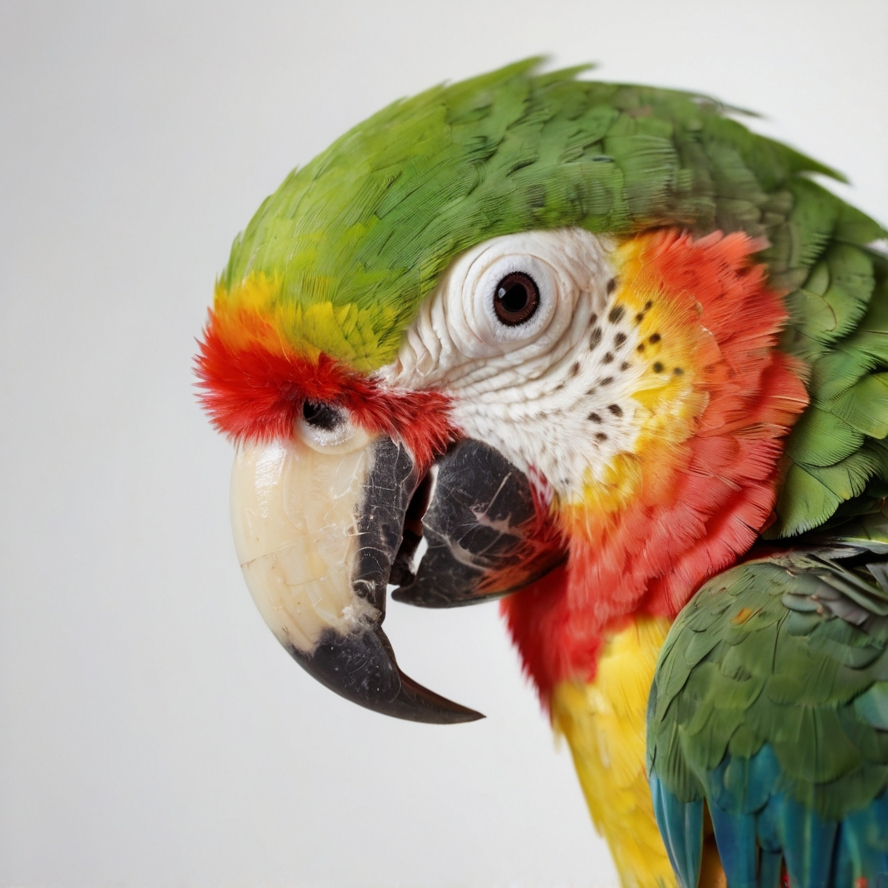
\includegraphics[width=2cm]{images/parrot4.jpg}};

\node[w=2cm, h=2cm, right=1cm of im1] (ie) {Image\\Encoder};
\begin{scope}[on behind layer]
 \draw[fill=mygreen!15] (ie.north west)--(ie.south west)--($(ie.south east)+(0,.3)$)--($(ie.north east)+(0,-.3)$)--cycle;   
\end{scope}
%----------
\matrix (m1) [right=1cm of ie, yshift=.6cm,
    matrix of nodes,
    column 1/.style={column sep=.2cm}, % Add gap after first column
    row 1/.style={row sep=.2cm},      % Add gap after first row
    row sep=-\pgflinewidth,
    column sep=-\pgflinewidth,
    nodes={
        draw,
        minimum width=1cm,
        minimum height=1cm,
        anchor=center,
        align=center
    }
] {
    % First row (empty first cell, then T values)
    & |[fill=myblue!15]| $T_1$ & |[fill=myblue!15]| $T_2$ & |[fill=myblue!15]| $T_3$ & |[fill=myblue!15]| $\cdots$ & |[fill=myblue!15]| $T_N$ \\
    % Second row
    |[fill=mygreen!15]| $I_1$ & $I_1T_1$ & $I_1T_2$ & |[fill=myred!15]| $I_1T_3$ & $\cdots$ & $I_1T_N$ \\
};

\node[below=1cm of m1-2-4, draw, w=2cm, h=1cm] (apo) {A photo of\\a bird.};
%---------
\node[w=2cm, h=2cm, above=2cm of ie] (ie1) {Image\\Encoder};
\begin{scope}[on behind layer]
 \draw[fill=mygreen!15] (ie1.north west)--(ie1.south west)--($(ie1.south east)+(0,.3)$)--($(ie1.north east)+(0,-.3)$)--cycle;   
\end{scope}

\node[left=1cm of ie1, draw, w=2cm, h=1cm] (apo1) {A photo of\\a (object).};

\node[draw, w=1.5cm, h=.6cm, left=1cm of apo1] (dog) {bird};
\node[draw, w=1.5cm, h=.6cm, above=0cm of dog] (car) {car};
\node[draw, w=1.5cm, h=.6cm, above=0cm of car] (plane) {plane};
\node[w=1.5cm, h=.6cm, below=0cm of dog] (dots) {$\vdots$\\[-1.5mm]};
\node[draw, w=1.5cm, h=.6cm, below=0cm of dots] (bird) {dog};

% Arrows
\draw[->] (im)--(a);
\draw[->] (a)--(a-|m.west);

\draw[->] (pta)--(te1);
\draw[->] (te1)-|(m-1-2);
\draw[->] (te1)-|(m-1-3);
\draw[->] (te1)-|(m-1-4);
\draw[->] (te1)-|(m-1-6);

\draw[->] (plane.east)--++(.5,0)|-(apo1);
\draw[->] (car.east)--++(.5,0)|-(apo1);
\draw[->] (dog.east)--++(.5,0)|-(apo1);
\draw[->] (bird.east)--++(.5,0)|-(apo1);

\draw[->] (apo1)--(ie1);

\draw[->] (ie1)-|(m1-1-2);
\draw[->] (ie1)-|(m1-1-3);
\draw[->] (ie1)-|(m1-1-4);
\draw[->] (ie1)-|(m1-1-6);

\draw[->] (m1-2-4)--(apo);
\draw[->] (im1)--(ie);
\draw[->] (ie)--(ie-|m1-2-1.west);

\node[anchor=south west, yshift=1cm] (l1) at (pta.north west) {\textbf{(1) Contrastive pre-training}};

\node[anchor=west] at (l1-|plane.north west) {\textbf{(2) Create dataset classifier from label text}};

\node[anchor=north west, yshift=-.7cm] (l3) at (bird.south west) {\textbf{(3) Use for zero-shot prediction}};

}
% }
\end{document}
